%{{{ Formatierung

\documentclass[a4paper,10pt]{article}

\usepackage{physics_notetaking}

%%% dark red
%\definecolor{bg}{RGB}{60,47,47}
%\definecolor{fg}{RGB}{255,244,230}
%%% space grey
%\definecolor{bg}{RGB}{46,52,64}
%\definecolor{fg}{RGB}{216,222,233}
%%% purple
%\definecolor{bg}{RGB}{69,0,128}
%\definecolor{fg}{RGB}{237,237,222}
%\pagecolor{bg}
%\color{fg}

\newcommand{\td}{\,\text{d}}
\newcommand{\RN}[1]{\uppercase\expandafter{\romannumeral#1}}
\newcommand{\zz}{\mathrm{Z\kern-.3em\raise-0.5ex\hbox{Z} }}
\newcommand{\id}{1\kern-.258em1}

\newcommand\inlineeqno{\stepcounter{equation}\ {(\theequation)}}
\newcommand\inlineeqnoa{(\theequation.\text{a})}
\newcommand\inlineeqnob{(\theequation.\text{b})}
\newcommand\inlineeqnoc{(\theequation.\text{c})}

\newcommand\inlineeqnowo{\stepcounter{equation}\ {(\theequation)}}
\newcommand\inlineeqnowoa{\theequation.\text{a}}
\newcommand\inlineeqnowob{\theequation.\text{b}}
\newcommand\inlineeqnowoc{\theequation.\text{c}}

\renewcommand{\refname}{Source}
\renewcommand{\sfdefault}{phv}
%\renewcommand*\contentsname{Contents}

\pagestyle{fancy}

\sloppy

\numberwithin{equation}{section}

%}}}


%{{{ Titelseite

\begin{document}

\begin{titlepage}
	\title{2 $|$ Diodenkennlinien}
	\author[1]{Angelo Brade\thanks{s72abrad@uni-bonn.de}}
	\author[1]{Jonas Wortmann\thanks{s02jwort@uni-bonn.de}}
	\affil[1]{Rheinische Friedrich--Wilhemls--Universität Bonn}
	\date{\today}
\end{titlepage}

\maketitle
\pagenumbering{gobble}

%}}}

\newpage

%{{{ Inhaltsverzeichnis

\fancyhead[R]{\thepage}
\fancyfoot[C]{}

\tableofcontents

%}}}

\newpage

%{{{

\pagenumbering{arabic}
\fancyhead[L]{\leftmark}

\section{Einleitung}
In diesem Versuch werden verschiedene Arten von Dioden und die mit ihnen zu bauenden Schaltungen untersucht.
Zudem werden Kennlinien von Dioden betrachtet und gemessen und Ein-- und Zweiweggleichrichterschaltungen mit Glättung behandelt.

%{{{ Theorie
\newpage
\section{Theorie}
\subsection{Halbleiter, Dotierung}
Halbleiter sind Materialien, zwischen deren Leitungs-- und Valenzband eine gewissen Gap--Energie ist.
Es ist Elektronen nicht möglich ohne die Aufnahme bzw.\ Abgabe von Energie, wie z.B.\ in Metallen, zwischen Valenz-- und Leitungsband zu wechseln.
\\Es gibt zwei Arten von Halbleitern bzw.\ --übergängen
\begin{enumerate}[label=--]
	\item Direkte Halbleiter: Wenn Energieminimum des Leitungsbands und Energiemaximum des Valenzbands direkt untereinander liegen, dann können Elektronen allein durch Aufnahme bzw.\ Abgabe eines Photons das Band wechseln.
	\item Indirekte Halbleiter: Wenn Energieminimum des Leitungsbands und Energiemaximum des Valenzbands nicht direkt untereinander liegen, sondern nuoch eine Verschiebung nach links oder rechts besitzen, dann müssen die Elektronen nicht nur ihre Energie mit Hilfe eines Photons ändern, sondern auch ihren Impuls durch Aufnahme eines Phonons.
\end{enumerate}
Es ist möglich Halbleiter zu dotieren.
Der Prozess der Dotierung beschreibt das Hinzufügen von gewollten Unreinheiten in einen Kristall, um die Leitungseigenschaften zu ändern.
Die p--Dotierung beschreibt das Hinzufügen von Atomen in ein Gitter, die ein Valenzelektron weniger als die Atome des Kristalls besitzen.
Das führt zu einem Ladungsüberschuss an \glqq positiven Ladungen\grqq{}, da nun eine freie Stelle im Gitter existiert, bei der Elektronen rekombinieren können.
Die n--Dotierung beschreibt das Hinzufügen von Atomen in ein Gitter, die ein Valenzelektron mehr als die Atome des Kristalls besitzen.
Das führt zu einem Ladungsüberschuss an negativen Ladungen, da diese Elektronen nicht mit anderen Atomen kombinieren.

\subsection{Dioden}
Dioden bestehen aus einem n-- und einem p--dotierten Material, welche eine Grenzschicht bilden und sind die einfachsten nichtlinearen Zweipole mit Kennlinie
\begin{figure}[h]
	\centering
	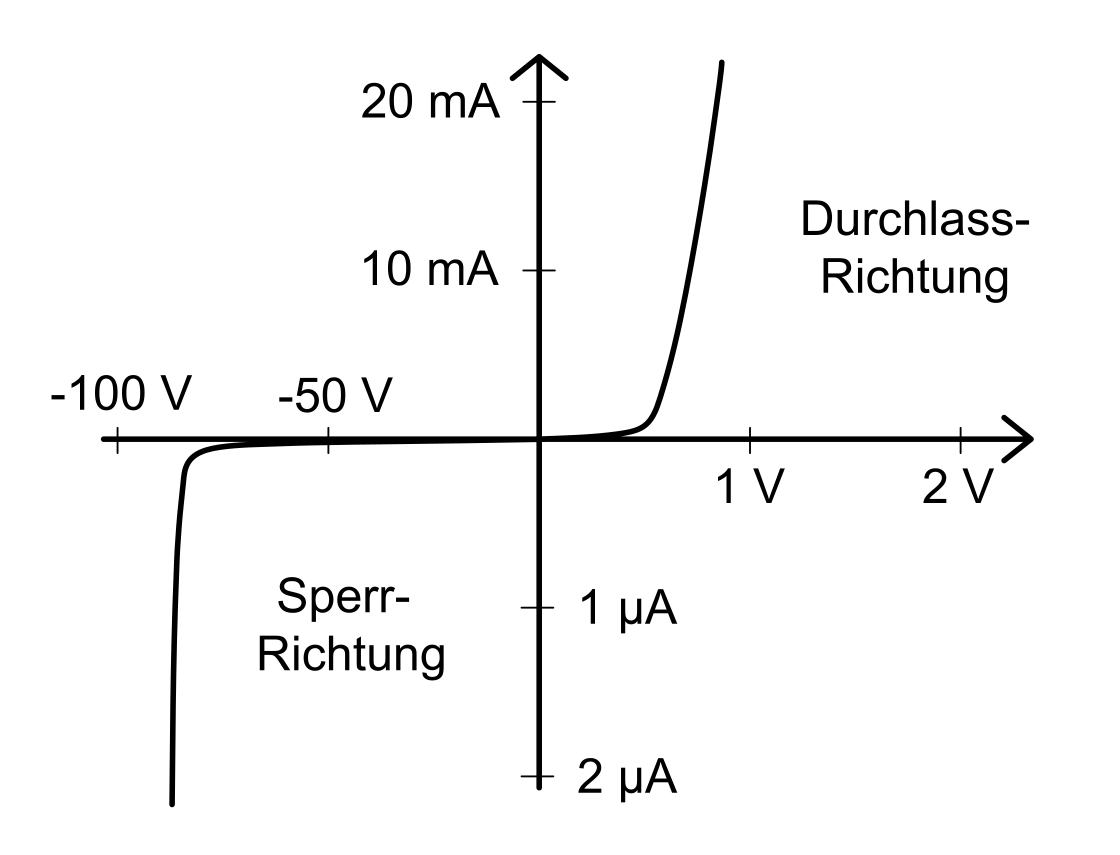
\includegraphics[width=0.4\textwidth]{diode_kennlinie.png}
	\caption{Kennlinie einer Diode; Abbildung 2.2 \cite{Praktikumsanleitung}}
\end{figure}\\
Es ist zu erkennen, dass die Diode Strom nur in eine Richtung fließen lässt.
In die Durchlassrichtung muss eine Mindestspannung von ca.\ $\SI{6}{V}$ bis $\SI{7}{V}$ anliegen, um das Gegenfeld der Diode zu überwinden.
Ist dieses Gegenfeld einmal überwunden, so kann ein großer Strom bei kleiner Spannung fließen.
In die Sperrichtung kommen meist nur wenige $\SI{}{\micro A}$ bei einer sehr hohen Spannung durch.

\subsection{Gleichrichter und Glättung}
Mit dieser Diode lassen sich Ein-- und Zweiweggleichrichter bauen, die Wechselspannung in direkte Spannung umwandeln.
\begin{figure}[h]
	\centering
	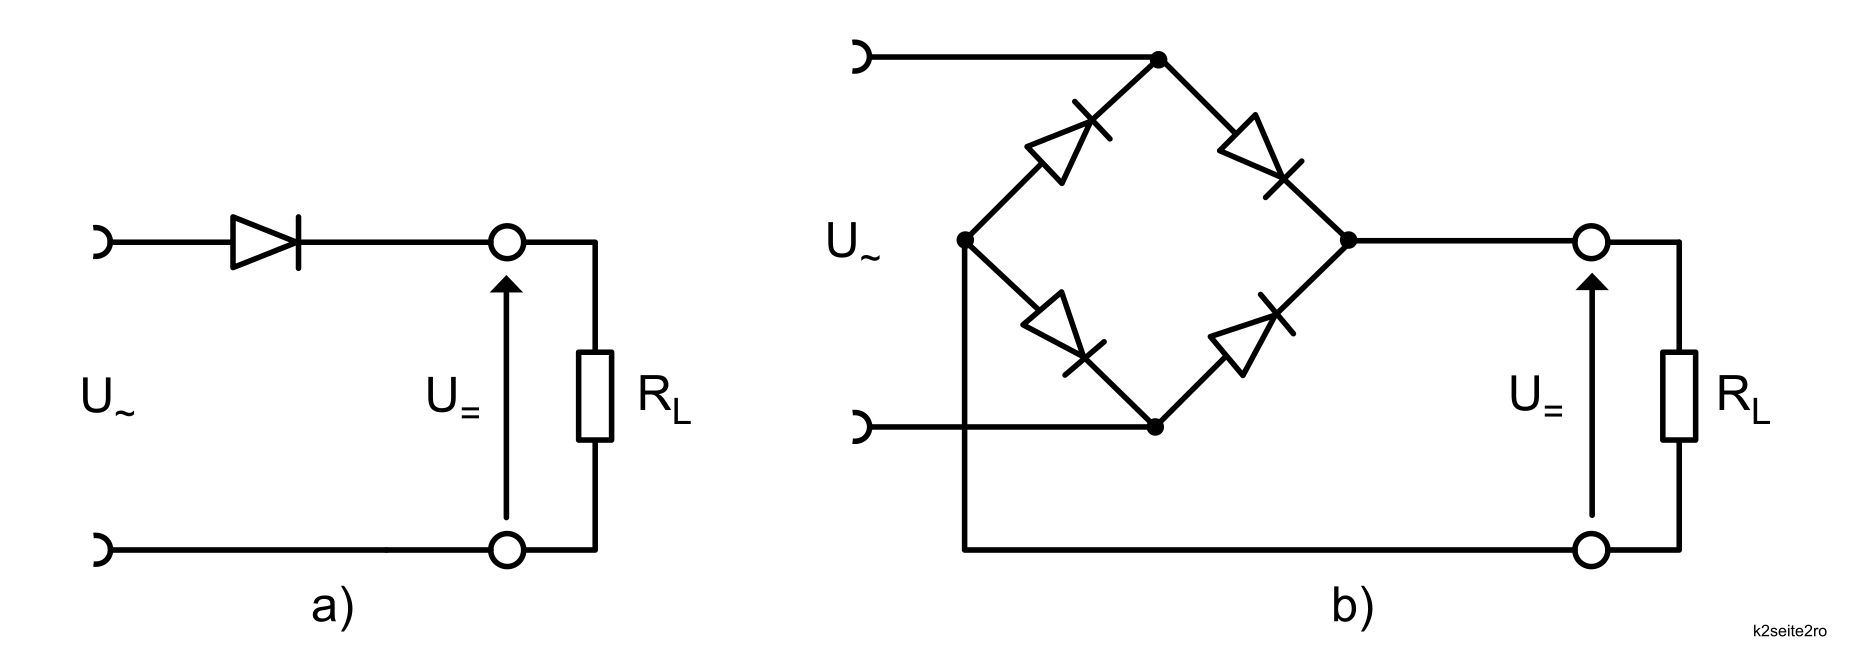
\includegraphics[width=0.7\textwidth]{ein_zweiweggleichrichter.png}
	\caption{Ein-- und Zweiweggleichrichter; Abbildung 2.4 \cite{Praktikumsanleitung}}
\end{figure}
Mit Hilfe eines Kondensators kann das noch vorhandene Brummen der Gleichspannung weitgehend unterdrückt werden.
Dieses existiert weiterhin, da Gleichrichter nur die Polarität der Spannung kompensieren und nicht interpolieren.
\begin{figure}[h]
	\centering
	\includegraphics[width=0.4\textwidth]{glättung.png}
	\caption{Glättungskondensator; Abbildung 2.5 \cite{Praktikumsanleitung}}
\end{figure}\\
Die Kapazität des Kondensators sollte möglichst so gewählt sein, dass die Restspannung ausreicht, um die Zeit zwischen den Wellen zu überbrücken, aber auch nicht zu groß, dass der Kondensator länger als ein Wellenberg auflädt.
Ist die Kapazität zu klein, so wird das Brummen weniger stark ausgeglichen und die Spannung fällt schneller ab.
%}}}

%{{{ Voraufgaben
\clearpage
\section{Voraufgaben}
\subsection{A}
Die Dicke der Grenzschicht eines p--n--Halbleiters ist bestimmt duch die Dichte der Dotierung.
Je höher die Dotierung auf der einen Seite der Grenzschicht ist, desto kleiner ist die Verarmungszone auf der anderen Seite.

\subsection{B}
Wird eine Spannung in Sperrrichtung einer Diode angelegt, so vergrößert sich die Grenzschicht, was dazu führt, dass sich die Kapazität der Diode verringert.

\subsection{C}
\begin{figure}[h]
	\centering
	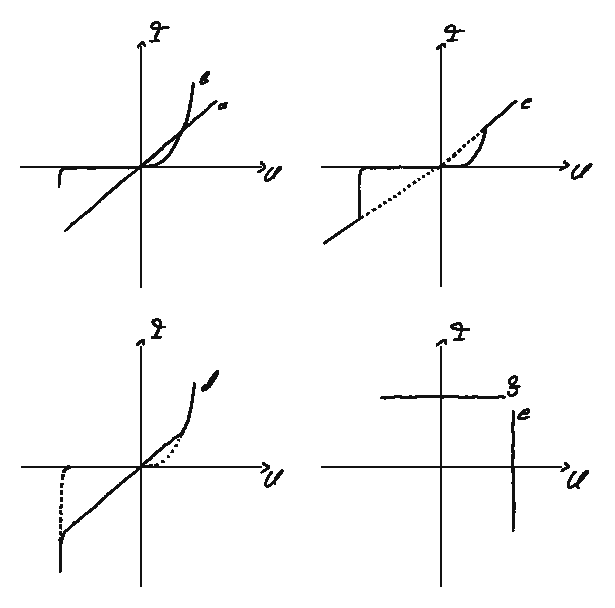
\includegraphics[width=0.7\textwidth]{C_crop.pdf}
	\caption[Kennlinienverlauf verschiedener Bauelemente]{Kennlinienverlauf verschiedener Bauelemente; $a$ \textsc{Ohm}'scher Widerstand, $b$ Diode, $c$ Diode und \textsc{Ohm}'scher Widerstand in Reihenschaltung, $d$ Diode und \textsc{Ohm}'scher Widerstand in Parallelschaltung, $e$ ideale Spannungsquelle, $f$ ideale Stromquelle}
\end{figure}
\noindent Die Widerstände in $c$ und $d$ sind jeweils verantwortlich für die Rück-- und Hinrichtung des Stroms, wenn sie in reihe oder parallel geschaltet sind.

\newpage
\subsection{D}
\begin{figure}[h]
	\centering
	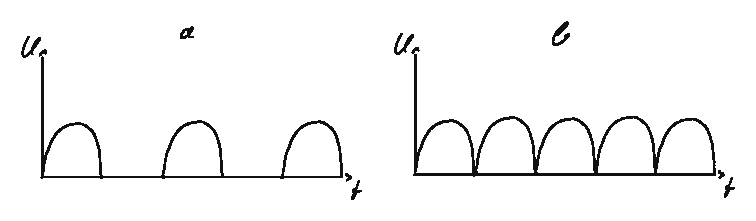
\includegraphics[width=\textwidth]{D_crop.pdf}
	\caption[Ein-- und Zweiweggleichrichter]{Ein-- und Zweiweggleichrichter mit einer Eingangsspannung weit über der Durchlassspannung.}
\end{figure}

\subsection{E}
Die Kapazität eines nach einem Gleichrichter geschalteten Kondensators muss so groß sein, dass sie über die Dauer, die die Spannung abfällt, ausreichend Energie gespeichert hat, um weiterhin eine konstante Spannung zu liefern.
Insofern sind größere Kapazitäten besser zum Ausgleich der Welligkeit.

\subsection{F}
Das Strommessgerät muss zur Messung der Kennlinie einer Diode in Durchlassrichtung \textit{hinter} der Diode und für die Kennlinie in Sperrrichtung \textit{vor} der Diode angeschlossen werden.
Das Spannungsmessgerät bleibt immer parallel zur Diode geschaltet.

\subsection{G}
Eine zum Strom proportionale Spannung lässt sich über einen \textsc{Ohm}'schen Widerstand herstellen, da die Relation
\begin{align}
	U=RI
\end{align}
gilt.

\subsection{H}
Die größte Kapazität eines Kondensators in einer Glättung mit einer Si--Diode ($I_{\text{max}}=\SI{1}{A}, U_{\text{max}}=\SI{400}{V})$ mit einer anliegenden Wechselspannung (Steigung von $\SI{0.01}{V.\micro s ^{-1}}$) liegt bei
\begin{align}
	C=\dfrac{Q}{U}=\dfrac{I\cdot \Delta t}{U}=\dfrac{\SI{1}{A}\cdot \SI{100}{\micro s}}{\SI{1}{V}}=\SI{100}{\micro F}
	.\end{align}

\subsection{I}
\begin{figure}[h]
	\centering
	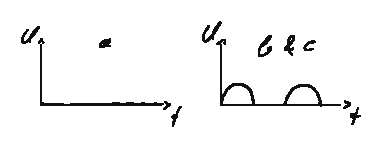
\includegraphics[width=0.8\textwidth]{I_crop.pdf}
	\caption[Ein-- und Zweigleichrichter (Variationen)]{Ein-- und Zweigleichrichter (Variationen)}
\end{figure}

\subsection{J}
Die Spannungs über das Potentiometer ergibt sich aus
\begin{align}
	U'=U_0\dfrac{R_L}{R_L+R}\label{eq:U'}
	.\end{align}
\begin{figure}[h]
	\centering
	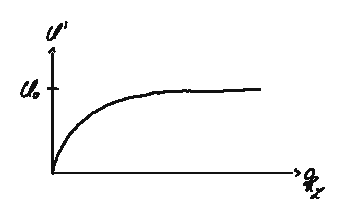
\includegraphics[width=0.5\textwidth]{J_crop.pdf}
	\caption[Spannungsabhängigkeit einer Spannungsteilerschaltung]{Spannungsabhängigkeit einer Spannungsteilerschaltung}
\end{figure}
Der Extremwert für $U'$ liegt bei $U_0$.

\subsection{K}
Für die Schaltung mit Zenerdiode gilt die Knotenregel
\begin{align}
	                &  & I                                                            & =I_{\text{ZD}}+I'                        &  & \\
	\Leftrightarrow &  & \dfrac{U}{R}                                                 & =I_{\text{ZD}}+\dfrac{U'}{R_{\text{L}} } &  & \\
	\Leftrightarrow &  & \dfrac{U_0-U_\text{ZD}}{R}                                   & =I_\text{ZD}+\dfrac{U'}{R_\text{L}}      &  & \\
	\Leftrightarrow &  & \dfrac{U_0-Z_\text{ZD}}{I_\text{ZD}+\tfrac{U'}{R_\text{L} }} & =R                                       &  &
	.\end{align}
Mit $U_0 \in \left[\SI{16}{V},\SI{22}{V}\right]$, $R_L \in \left[\SI{200}{\ohm},\infty\,\SI{}{\ohm}\right]$, $I_\text{ZD} \in \left[\SI{2}{\milli A},\SI{100}{mA}\right]$  und $U'=\SI{8.2}{V}$ liegt der Wertebereich für den Widerstand bei
\begin{align}
	R \in \left[\SI{138}{\ohm},\SI{182}{\ohm}\right]
	.\end{align}
%}}}

\clearpage
\section{Auswertung}
\subsection{Versuchsaufgabe 1: Statistische Messung der Diodenkennlinie}
Für die Siliziumdiode MRA4004 und die \textsc{Schottky}diode 10BQ015 wird mit einer statistischen Messung mit Hilfe von Strom-- und Spannungsmessgerät die Kennlinie geplottet.
Dazu werden die Dioden des Diodenschaltbretts verwendet

\subsection{Versuchsaufgabe 2: Oszillogramm der Diodenkennlinie}
Wir zeichen die Kennlinie als Oszillogramm von der Silizium-, Schottky- und Zener-Diode auf. Dies wird mithilfe einer Schaltung, die im Abschnitt "Versuchsaufgabe 2: Oszillogramm der Diodenkennlinie" \cite{Praktikumsanleitung} beschrieben wird, aufgebaut. An dieser Stelle sei angemerkt, dass es starke Probleme bezüglich des Aufbaus gab und uns von Asistenten geholfen wurde. Das Hauptproblem hat sich als eine Defekte "Black Box" \cite{Praktikumsanleitung} herrausgestellt, welche eigentlich den Strom wiedergeben sollte. Die Kennlinien sind für die Siliziumdiode in Abb. \ref{fig:2.1}, für die Schottkyiode in Abb. \ref{fig:2.2} und für die Zenerdiode Abb. \ref{fig:2.3} und \ref{fig:2.4} zu sehen.

\newpage
\begin{figure}[h]
	\centering
	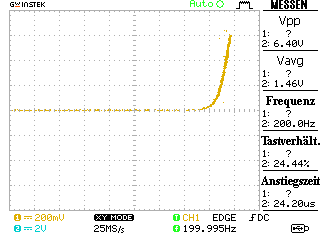
\includegraphics[width=0.6\textwidth]{data/Kennlinie_a1_d1.BMP.png}
	\caption{Kennlinie der Siliziumdiode MRA4004; max.\ Sperrspannung $\SI{400}{V}$; max.\ Durchlassstrom $\SI{1000}{mA}$}.
	\label{fig:2.1}
\end{figure}
\begin{figure}[h]
	\centering
	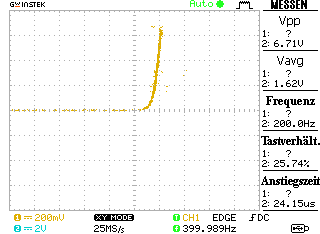
\includegraphics[width=0.6\textwidth]{data/Kennlinie_a1_d2.BMP.png}
	\caption{Kennlinie der \textsc{Schottky}diode 10BQ015; max.\ Sperrspannung $\SI{15}{V}$; max.\ Durchlassstrom $\SI{1000}{mA}$}
	\label{fig:2.2}
\end{figure}
\begin{figure}[h]
	\centering
	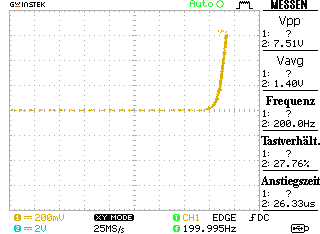
\includegraphics[width=0.6\textwidth]{data/Kennlinie_a1_zd.BMP.png}
	\caption{Kennlinie der Zenerdiode}
	\label{fig:2.3}
\end{figure}
\begin{figure}[h]
	\centering
	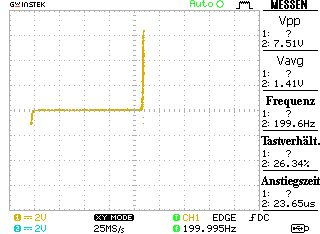
\includegraphics[width=0.6\textwidth]{data/Kennlinie_a1_zd_fern.BMP.png}
	\caption{Kennlinie der Zenerdiode mit 10-facher Verkleinerung der x-Achse}
	\label{fig:2.4}
\end{figure}
Wir erkennen, dass die Schottkydiode eine deutlich früher anfangende Durchlassspannung von ca. 60(12) mV hat, wobei die Siliziumdiode und Zenerdiode eine Durchlassspannung von ca. 560(12) mV haben. Dies ist ein deutliches Merkmal jeder Schottkydiode, da diese aus einem Halbleiter und einem Metall besteht, anstelle von zwei verschieden dotierten Halbleitern. Den zweiten Unterschied erkennen wir, wenn wir die Abb. \ref{fig:2.4} betrachten. Dort können wir einen Durchbruch bei der Zenerspannung von -800(12) mV erkennen. Ein praktisch wertvolles Merkmal ist hierbei, dass die Diode nicht zerstört wird. Ein verkleinertes Bild der Siliziumdiode, sowie Schottkydiode ist an dieser Stelle sinfrei, da wir die Sperrspannung von -400 V und -15 V mit einer Maximalausgangsspannung von 15 V nicht erreichen.


\subsection{Versuchsaufgabe 4: Oszillogramm des Zweiweggleichrichters}
Wir verbauen im Vergleich zu Versuchsaufgabe 3 nun aber anstatt des Einweggleichrichters den Zweiwegleichrichter. Wir erhalten die in Abb. \ref{fig:4.1} gezeigte Spannung ohne den Kondensator, Abb. \ref{fig:4.2} mit 2.2µF, Abb. \ref{fig:4.3} mit 22 µF und Abb. \ref{fig:4.4} mit 1000µF.
\begin{figure}[h]
	\centering
	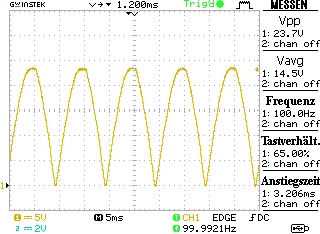
\includegraphics[width=0.6\textwidth]{data/a4_a.BMP.png}
	\caption{Oszillogramm eines Zweiweggleichrichters ohne Kondensator}
	\label{fig:4.1}
\end{figure}
\begin{figure}[h]
	\centering
	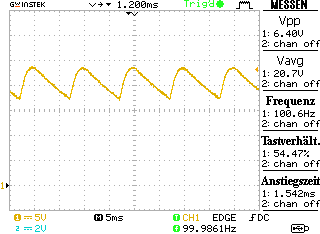
\includegraphics[width=0.6\textwidth]{data/a4_b.BMP.png}
	\caption{Oszillogramm eines Zweiweggleichrichters mit 2.2 µF Kondensator}
	\label{fig:4.2}
\end{figure}
\begin{figure}[h]
	\centering
	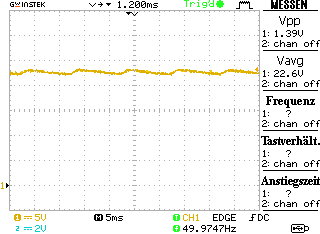
\includegraphics[width=0.6\textwidth]{data/a4_c.BMP.png}
	\caption{Oszillogramm eines Zweiweggleichrichters mit 22 µF Kondensator}
	\label{fig:4.3}
\end{figure}
\begin{figure}[h]
	\centering
	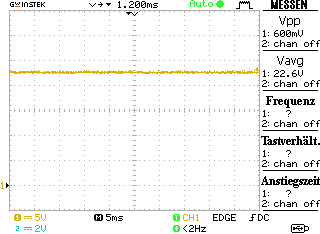
\includegraphics[width=0.6\textwidth]{data/a4_d.BMP.png}
	\caption{Oszillogramm eines Zweiweggleichrichters mit 1000 µF Kondensator}
	\label{fig:4.4}
\end{figure}
Hier sei darauf Hingewiesen, dass die Zeitskalierung halbiert wurde, sodass es den fälschlichen Anschein erweckt, dass die Schwingung breiter geworden sei. Eigentlich sind aber jetzt die vorher beim Einweggleichrichter gesperrten und Ursprünglich negativen Spannungen umgepolt worden, sodass es zwischen jeder Ursprünglichen positiven Spannungsschwankung nun einen weiteren Spannungsberg gibt.
Es ist deutlich zu erkennen, wie mit steigener Kapazität die Brummspannung sich verringert. Ohne Kondensator gibt es keine Abflachung und mit dem 1000 µF Kondensator gibt es volle Abflachung, also es ist kein Brumm mehr zu erkennen.

\begin{center}
	\begin{tabular}{|c|c|c|}
		\hline
    \(C \) [µF] & \(U_{\text{PP}}\) [V] & \(U_{\text{avg}}\) [V]\\
		\hline
    0.0 & 23.7 & 14.5\\
    2.2 & 6.4 & 20.7 \\
    22 & 1.39 & 22.6 \\
    1000 & 0.6 & 22.6 \\
		\hline
	\end{tabular}
	\captionof{table}{Brummspannung und mittlere Höhe der Gleichspannung gegenüber der Kapazitäten der verschiedenen Kondensatoren}
	\label{Tab:4.1}
\end{center}

Vergleichsweise zum Einweggleichrichter, sind die weiteren Spannungsberge durch die Invertierung des Signals, dank des Zweiweggleichrichters zu erklären. Es sind nochmal alle Brummspannungen, sowie die mittleren Höhen der Gleichspannungen mit der entsprechenden Kapazität in Tabell \ref{Tab:4.1} einzusehen.

\section{Fazit}
Wir haben mit der ersten Versuchsaufgabe Kennlinien mittels Amperemeter und Voltmeter vermessen und konnten dort schon den späteren Anstieg der Durchlassspannung der Silizium- gegenüber der Schottky-Diode sehen. Dies konnten wir nochmal in der zweiten Versuchsaufgabe mittels Oszillogramms bestätigen, sowie bei der Zenerdiode eine Zenerspannung von -800(12) mV messen, die deutlich unter der Sperrspannung von -400V und -15V der anderen Dioden liegt. Desweiteren haben wir den Einweggleichrichter untersucht, bei dem wir auch stärkere Glättungen durch höhere Kapazitäten erzeugen konnten. Dieses Verhalten wurde dann nochmal in der nächsten Versuchsaufgabe mit dem Zweiweggleichrichter bestätigt, wobei wir zudem noch die negativen Spannungen invertiert haben. Im letzten Versuchsteil haben wir dann mithilfe einer Zenerdiode ein Singal stabilisiert.
 
\clearpage
\listoffigures
\listoftables
\bibliographystyle{plain}
\bibliography{refs}

%}}}

\end{document}
